\documentclass[11pt]{article}
\usepackage[a4paper,margin=0.82in]{geometry}
\usepackage{fontspec}
\usepackage{xeCJK}
\usepackage{graphicx}
\usepackage{booktabs}
\usepackage{caption}

\setmainfont{Times New Roman}
\setsansfont{Arial}
\setCJKmainfont{Songti SC}
\setCJKsansfont{STHeiti}
\setlength{\parskip}{0.62em}
\setlength{\parindent}{0pt}

\title{Traditional 与 Learning-based 事件表示对比报告}
\author{}
\date{2026-05-08}

\begin{document}
\sloppy
\maketitle

\paragraph{Protocol Alignment.} 本版报告将 N-MNIST learning-based 结果更新为完整 GPU aligned run，因此 N-MNIST 中 7 个 learning-based 方法和 5 个 traditional 方法现在可以放入同一张正式 accuracy 图中比较。N-MNIST 采用官方 train/test split，learning-based 运行设置为 RTX 4090、100 epoch 上限、early stopping patience 10、batch size 32、learning rate 0.0001、weight decay 0.0001 和 seed 42；traditional baseline 采用已记录的官方 test set 结果。N-Caltech101 与 MVSEC 沿用仓库已有结果，其中 MVSEC 是 outdoor\_day1/2 训练、indoor\_flying1/2/3 测试的统一 optical-flow protocol。

\begin{figure}[t]
  \centering
  
\includegraphics[width=0.90\linewidth]{nmnist_accuracy_full_aligned.pdf}
  \caption{N-MNIST 完整官方测试集准确率对比。蓝色为 learning-based 方法，橙色为 traditional baseline。}
  \label{fig:nmnist-acc}
\end{figure}

\paragraph{N-MNIST Is Saturated But Now Comparable.} 在完整 N-MNIST setting 下，最佳方法是 Matrix-LSTM，test accuracy 为 99.40\%。最佳 learning-based 方法 Matrix-LSTM 为 99.40\%，最佳 traditional 方法 Voxel Grid 为 99.08\%，差距为 0.32 个百分点。除 Binary Event Image 外，大多数方法集中在 98.18--99.40\% 区间，说明 N-MNIST 已接近饱和，适合验证 pipeline 和基本表示能力，但不适合单独作为强结论来源。最弱方法 Binary Event Image 为 95.06\%，主要说明完全二值化的事件投影会丢失可见信息。

\begin{figure}[t]
  \centering
  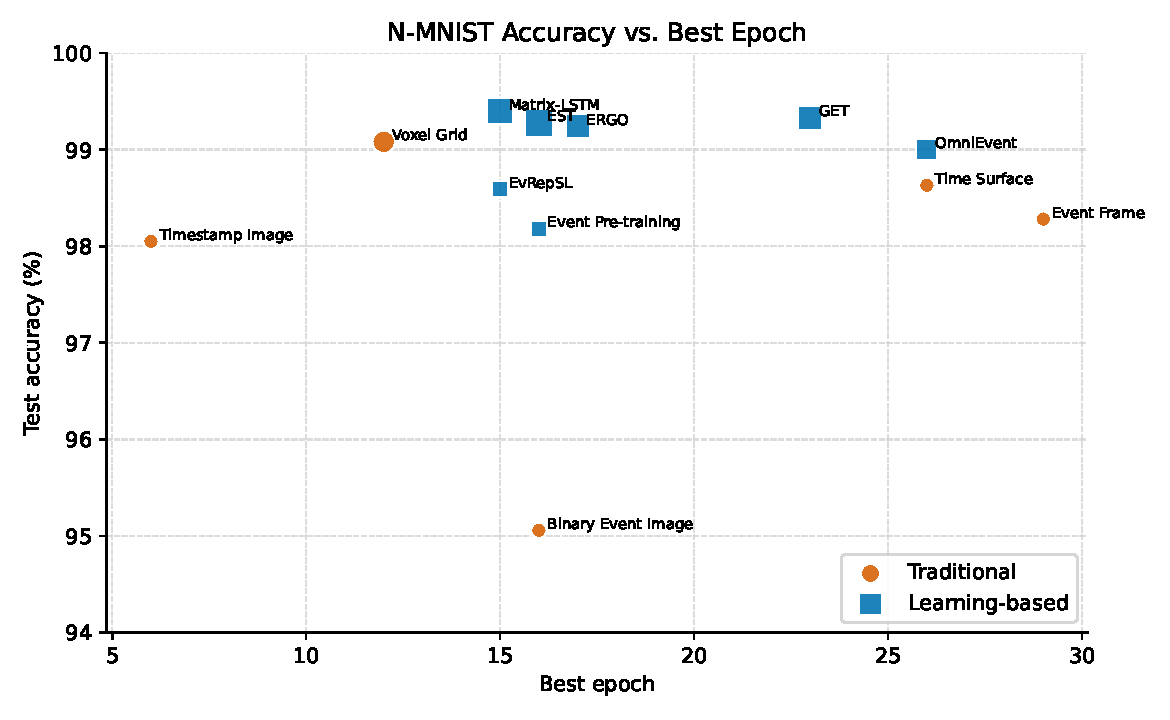
\includegraphics[width=0.88\linewidth]{nmnist_accuracy_epoch_scatter.pdf}
  \caption{N-MNIST 准确率与最佳 epoch 的关系。点大小随输入通道数变化，用于展示表示维度、收敛位置和准确率之间的权衡。}
  \label{fig:nmnist-eff}
\end{figure}

\paragraph{Accuracy-Efficiency Trade-off.} N-MNIST 的 best epoch 显示出比最终准确率更有区分度的模式。Learning-based 方法大多在第 15--26 epoch 取得最佳结果，其中 Matrix-LSTM 在第 15 epoch 达到 99.40\%，GET 在第 23 epoch 达到 99.33\%，EST 在第 16 epoch 达到 99.28\%。Traditional 方法中 Timestamp Image 的最佳 epoch 仅为 6，准确率仍有 98.05\%；Voxel Grid 在第 12 epoch 达到 99.08\%。这说明更复杂或多通道的表示未必总是需要更长训练，但在 N-MNIST 这种饱和任务中，小幅准确率提升通常伴随更高表示维度或更复杂 adapter。

\begin{figure}[t]
  \centering
  
\includegraphics[width=0.92\linewidth]{ncaltech101_accuracy_full_aligned.pdf}
  \caption{N-Caltech101 分类准确率对比。该任务比 N-MNIST 更能拉开 representation capacity 的差异。}
  \label{fig:ncaltech}
\end{figure}

\paragraph{N-Caltech101 Reveals Larger Capacity Gaps.} N-Caltech101 的结果与 N-MNIST 不同。当前最佳 learning-based 方法 EST adaptation 为 70.44\%，最佳 traditional 方法 Timestamp Image 为 52.93\%，差距达到 17.51 个百分点。这个差距比 N-MNIST 明显得多，说明在类别数更多、形状变化更复杂的分类任务上，learning-based representation 更能利用事件流中的跨时间结构；traditional 方法在此处更适合作为非学习表示下界和计算成本参照。

\begin{figure}[t]
  \centering
  
\includegraphics[width=0.88\linewidth]{mvsec_aee_full_aligned.pdf}
  \caption{MVSEC optical flow 统一协议 AEE 对比。AEE 越低越好，横轴采用局部放大。}
  \label{fig:mvsec}
\end{figure}

\paragraph{MVSEC Gives A Counterpoint.} MVSEC optical flow 结果提供了与分类任务不同的证据。在统一 decoder 和统一 early-stopping protocol 下，最佳方法是 Timestamp Image，AEE 为 2.7916，outlier rate 为 36.61\%；最佳 learning-based 方法 EST 的 AEE 为 2.8654。这说明 timestamp-preserving traditional representation 在 dense motion estimation 中仍然很强。严谨表述应是：在本仓库统一 optical-flow protocol 下，Timestamp Image 优于当前 learning-based 最优结果；这不等价于否定 learning-based 方法在其原论文完整系统中的潜力。

\paragraph{Takeaway For Presentation.} 当前证据支持一个分任务结论。N-MNIST 上两类方法都接近天花板，最佳 learning-based 只比最佳 traditional 高 0.32 个百分点，因此不应过度解读微小排名；N-Caltech101 上 learning-based 优势清晰，最佳方法比最佳 traditional 高 17.51 个百分点；MVSEC 上 traditional Timestamp Image 在统一协议下取得最低 AEE，说明传统事件表示不是弱 baseline。汇报时可以强调：传统方法在简单分类和光流估计中仍然具有竞争力，而 learning-based 方法在更复杂分类任务中展现出更强的表示容量。

\end{document}
